\section{设计思想}
% 本程序中用到的所有数据类型的定义,主程序的流程图及各程序模块之间的调用关系
\subsection{逻辑设计}
\subsubsection{链表}

\begin{figure}[H]
    \begin{minipage}[c]{0.5\linewidth}
        \centering
        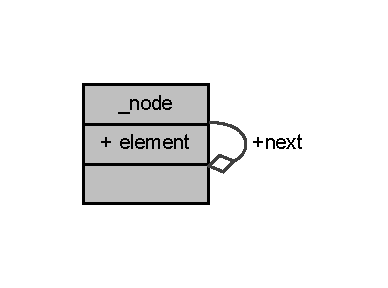
\includegraphics[width=\linewidth]{figures/struct__node}
        \caption{链表节点}
        \label{fig:structnode}
    \end{minipage}
    \begin{minipage}[c]{0.5\linewidth}
        \begin{lstlisting}[language = c]
typedef void *ElementPtr;

struct _node {
  ElementPtr element;
  struct _node *next;
};

typedef struct _node *PtrNode;
typedef PtrNode List;
typedef PtrNode Position;
        \end{lstlisting}
    \end{minipage}
\end{figure}

\textbf{主要操作}

\lstinputlisting[language = c]{../list.h}

\subsubsection{多项式}
\begin{figure}[H]
    \begin{minipage}[c]{0.25\linewidth}
        \centering
        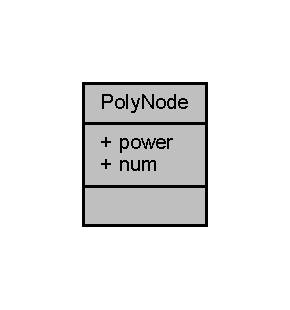
\includegraphics[width=\linewidth]{figures/struct_poly_node}
        \caption{多项式节点}
        \label{fig:structnode}
    \end{minipage}
    \begin{minipage}[c]{0.3\linewidth}
        \centering
        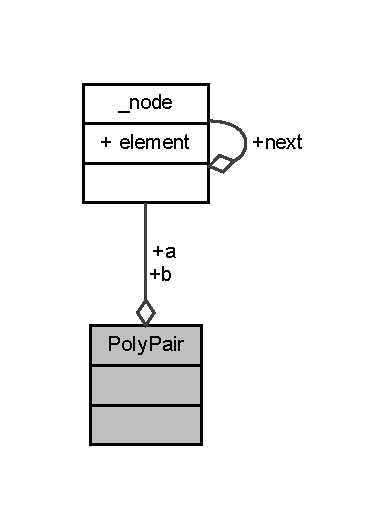
\includegraphics[width=\linewidth]{figures/struct_poly_pair}
        \caption{Pair}
        \label{fig:structnode}
    \end{minipage}
    \begin{minipage}[c]{0.4\linewidth}
        \begin{lstlisting}[language = c]
typedef List Poly;

typedef struct PolyNode {
  int power;
  int num;
} *PolyNode;

typedef struct PolyPair {
  Poly a;
  Poly b;
} PolyPair;
        \end{lstlisting}
    \end{minipage}
\end{figure}

\textbf{内存频繁申请解决方案}

\begin{lstlisting}[language = c]
    static List AvaList = NULL;

    void DeleteNode(PtrNode node) {
    // 将element域的内存释放并入AvaList
    node->next = First(AvaList);
    free(node->element);
    AvaList->next = node;
    }

    void FreeMem() {
    // 将可用空间表内存全部释放
    _DeleteList(AvaList);
    }

    static PtrNode GetAva() {
    // 如果为空就分配内存,否则返回可用空间
    if (AvaList == NULL) {
    AvaList = CreateList();
    //程序终止时完全释放内存
    atexit(FreeMem);
    }
    PtrNode node = First(AvaList);
    if (node != NULL)
    AvaList->next = node->next;
    else
    node = (PtrNode) malloc(sizeof(struct _node));
    return node;
    }
\end{lstlisting}

\textbf{主要操作}

\lstinputlisting[language = c]{../polynomial.h}

\subsubsection{整体依赖关系图}

\begin{figure}[H]
    \centering
    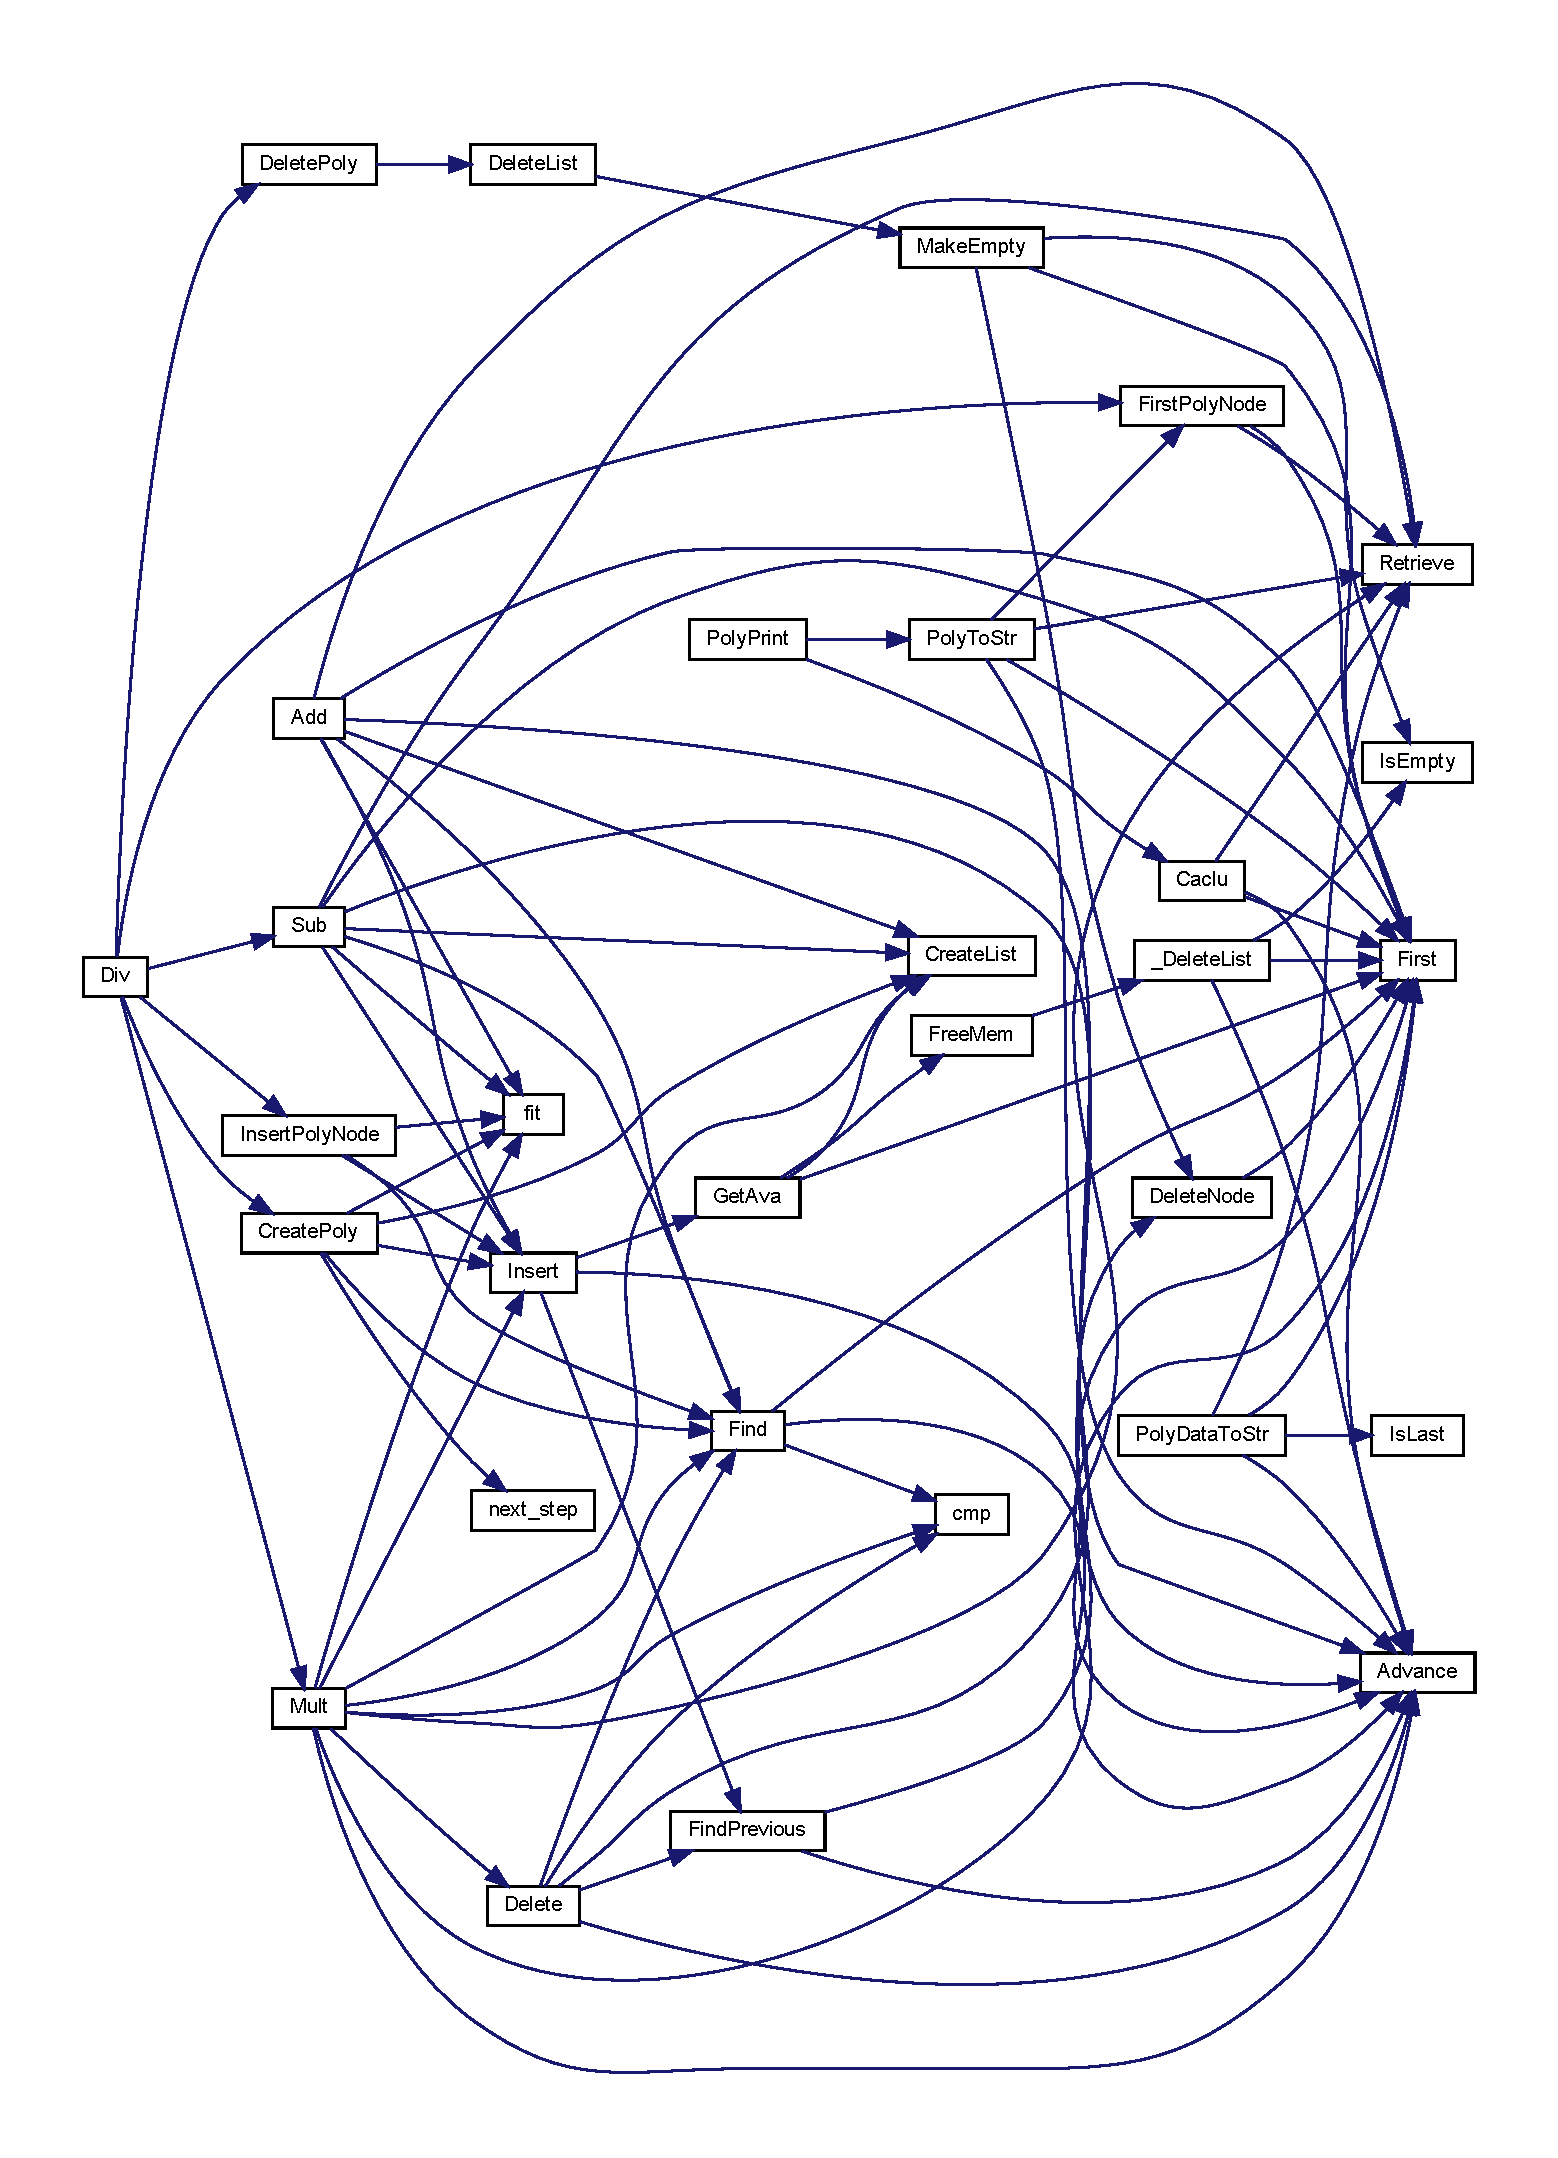
\includegraphics[width=0.9\linewidth]{figures/call_graph}
    \caption{整体依赖关系图}
    \label{fig:callgraph}

\end{figure}



\subsection{Main函数流程图}
\begin{figure}[H]
    \centering
    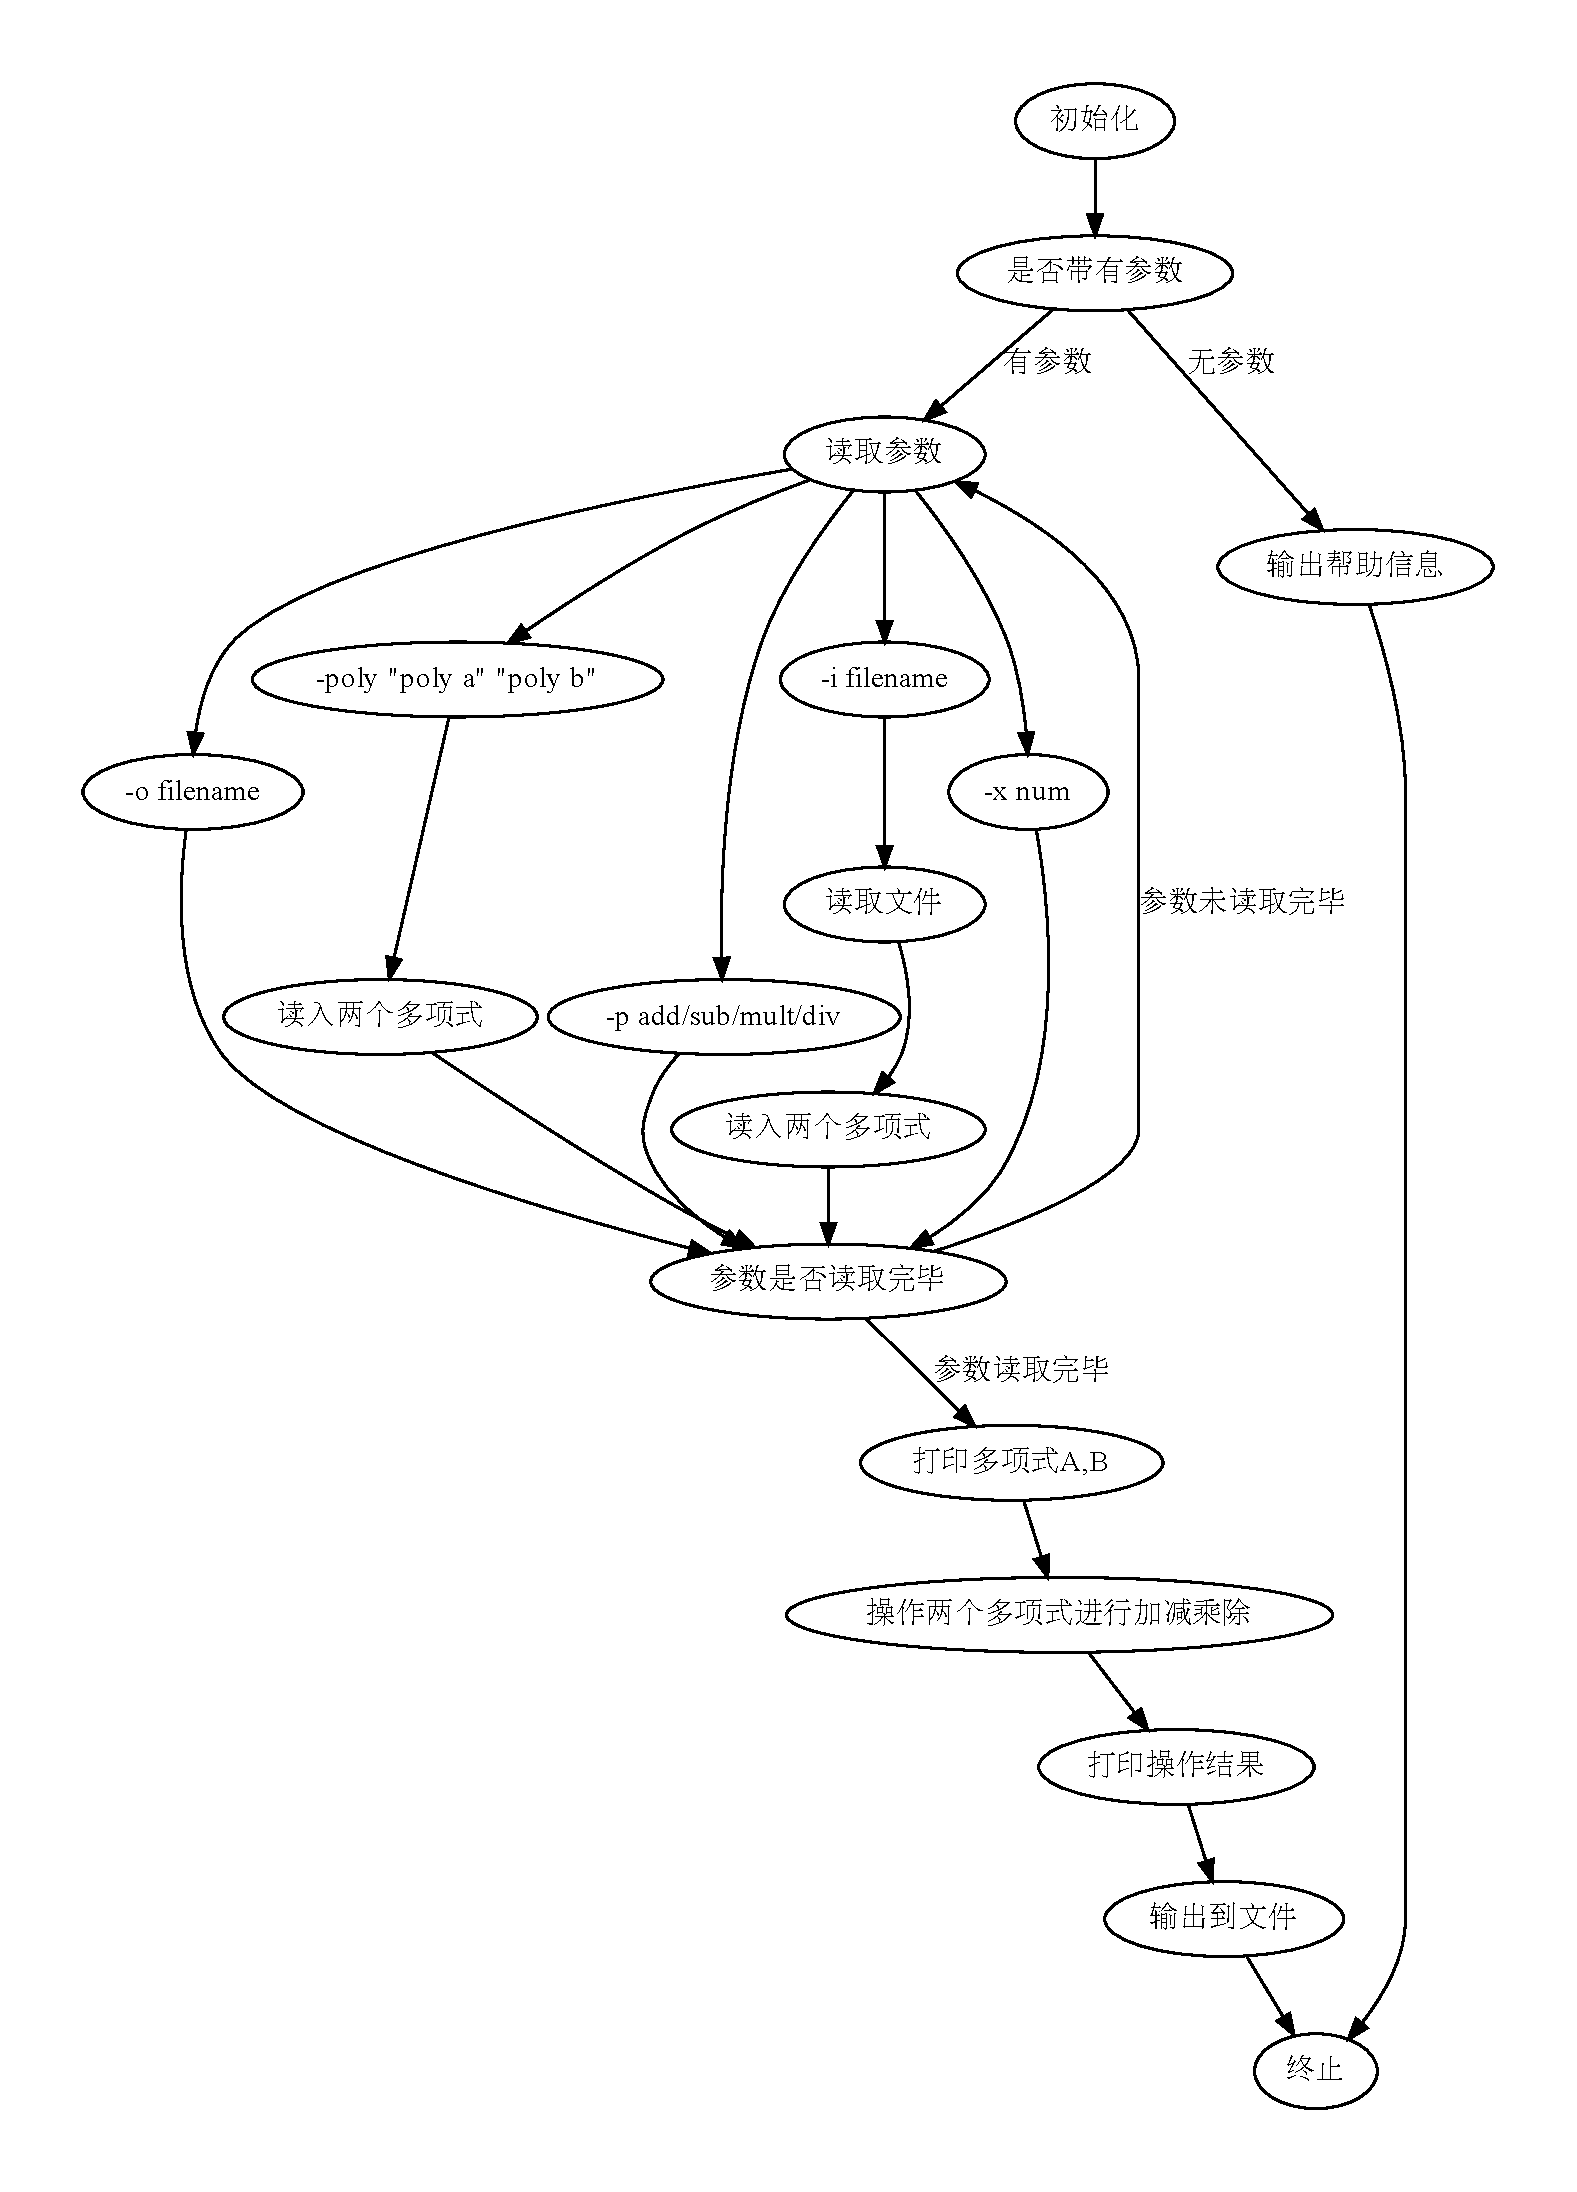
\includegraphics[width=0.7\linewidth]{figures/main}
    \caption{主函数流程图}
    \label{fig:main}
\end{figure}